% ==========================================================================
% fig_module3_schematic_compact.tex -> Panel A (for the Fig 3 2x2 composite)
% Genetic & Exposomic Mediation (GEM): TWO driver paths (genetic, exposomic),
% each decomposed into a direct (NDE) and an indirect (NIE) effect through the
% protein. NIE_k = (driver->protein) x (protein->disease); TE_k = NDE_k + NIE_k;
% PM_k = NIE_k / TE_k. Colour carries the payload (genetic=blue, exposome=orange,
% protein=green, disease=red); direct paths dashed/muted. Compact top-left inset.
% Build: tectonic --outdir <dir> fig_module3_schematic_compact.tex
%        pdftocairo -png -r 300 -singlefile <pdf> <out>
% ==========================================================================
\documentclass[border=6pt]{standalone}
\usepackage{fontawesome5}
\usepackage{xcolor}
\usepackage{tikz}
\renewcommand{\familydefault}{\sfdefault}
\hyphenpenalty=10000\exhyphenpenalty=10000
\usetikzlibrary{shapes.geometric,arrows.meta,positioning,backgrounds,fit,calc,shadows.blur}
\definecolor{ink}{HTML}{1F2937}\definecolor{mute}{HTML}{6B7280}
\definecolor{gen}{HTML}{1B6CA8}\definecolor{genl}{HTML}{7FB3D5}
\definecolor{expo}{HTML}{E07B39}\definecolor{prot}{HTML}{1B7837}
\definecolor{dz}{HTML}{B2182B}
\definecolor{palegen}{HTML}{E7F0F7}\definecolor{paleexpo}{HTML}{FCEDE1}
\definecolor{paleprot}{HTML}{E7F3EB}\definecolor{paledz}{HTML}{FAE8EA}
\begin{document}
% Compact GEM concept inset: two driver paths, each NDE + NIE.
\begin{tikzpicture}[font=\sffamily,>={Stealth[round]},
  drv/.style={rectangle,rounded corners=2.5pt,line width=0.8pt,align=center,inner sep=3pt,
    minimum width=2.0cm,minimum height=0.78cm},
  org/.style={circle,line width=0.9pt,align=center,inner sep=1pt,minimum size=1.3cm},
  plab/.style={align=center,font=\scriptsize,text=ink},
  tag/.style={font=\tiny\bfseries,fill=white,inner sep=1.1pt},
  nieG/.style={line width=1.2pt,draw=gen},
  nieE/.style={line width=1.2pt,draw=expo},
  nieP/.style={line width=1.2pt,draw=prot},
  ndeG/.style={line width=0.8pt,draw=gen,dash pattern=on 2.5pt off 1.8pt},
  ndeE/.style={line width=0.8pt,draw=expo,dash pattern=on 2.5pt off 1.8pt}]

% --- title (compact, no subtitle) ---
\node[anchor=west,font=\bfseries\small,text=ink] at (-0.05,3.96)
  {Genetic \& Exposomic Mediation \textcolor{mute}{(GEM)}};

% --- driver boxes (left): genetics + exposome each mediate independently ---
\node[drv,draw=gen,fill=palegen,text=gen] (G) at (1.05,2.62)
  {\textbf{\faDna~Genetics}};
\node[drv,draw=expo,fill=paleexpo,text=expo] (E) at (1.05,0.95)
  {\textbf{\faLeaf~Exposome}};

% --- protein + disease ---
\node[org,draw=prot,fill=paleprot,text=prot] (P) at (3.62,1.80)
  {{\faVial}\\[-1pt]{\tiny\textbf{Protein}}};
\node[org,draw=dz,fill=paledz,text=dz] (D) at (6.12,1.80)
  {{\faHeartbeat}\\[-1pt]{\tiny\textbf{Disease}}};

% --- indirect (NIE): each driver -> protein limb is its own NIE; the protein ->
% disease step is shared. NIE_k = (driver->protein) x (protein->disease). ---
\draw[nieG,->] (G.east) to[out=0,in=150]
  node[tag,text=gen,pos=0.52,yshift=4pt]{NIE$_{\!G}$} (P.150);
\draw[nieE,->] (E.east) to[out=0,in=210]
  node[tag,text=expo,pos=0.52,yshift=-4pt]{NIE$_{\!E}$} (P.210);
\draw[nieP,->] (P.east) -- (D.west);

% --- direct (NDE): genetics arcs OVER the top, exposome UNDER the bottom (both
% bypass the protein, non-crossing), each its own NDE. ---
\draw[ndeG,->] (G.40) to[out=42,in=124]
  node[tag,text=gen,pos=0.55]{NDE$_{\!G}$} (D.116);
\draw[ndeE,->] (E.south) to[out=-90,in=246]
  node[tag,text=expo,pos=0.86]{NDE$_{\!E}$} (D.254);

% --- decomposition formula (bottom, per-driver, two lines) ---
\node[rectangle,rounded corners=2pt,draw=mute,fill=black!3,inner sep=4pt,
  font=\scriptsize,text=ink,anchor=north,align=center] at (3.05,-0.32)
  {\textbf{TE}$_k$ $=$ \textcolor{mute}{NDE$_k$} $+$ \textcolor{prot}{NIE$_k$}
     \quad\textbf{PM}$_k$ $=$ \textcolor{prot}{NIE$_k$}\,$/$\,TE$_k$\\[2pt]
   {\tiny\textcolor{mute}{NDE$_k$, NIE$_k$ by g-computation (counterfactual mediator, 1-SD change in driver $k$);\;\;
     $k\in\{$\textcolor{gen}{G}, \textcolor{expo}{E}$\}$}}};
\end{tikzpicture}
\end{document}
